% This is samplepaper.tex, a sample chapter demonstrating the
% LLNCS macro package for Springer Computer Science proceedings;
% Version 2.20 of 2017/10/04
%
\documentclass[runningheads]{llncs}
%
\usepackage[pdftex]{graphicx}
\usepackage{gensymb}
% Used for displaying a sample figure. If possible, figure files should
% be included in EPS format.
%
% If you use the hyperref package, please uncomment the following line
% to display URLs in blue roman font according to Springer's eBook style:
% \renewcommand\UrlFont{\color{blue}\rmfamily}

\usepackage{xcolor}
\usepackage{caption} %needed to make captions on figure* centered
\graphicspath{{./figures/}}
\DeclareGraphicsExtensions{.pdf,.png}
\usepackage[bookmarks=false]{hyperref}
\usepackage[linesnumbered, ruled, vlined]{algorithm2e}

% correct bad hyphenation here
\hyphenation{}


\begin{document}
%

\title{Sparta: A Heat Budget-based Scheduling Framework on Edge Devices for Machine Learning Applications}
%
%\titlerunning{Abbreviated paper title}
% If the paper title is too long for the running head, you can set
% an abbreviated paper title here
%


\author{Michael Zhang\inst{1} \and
Chandra Krintz\inst{1} \and
Rich Wolski\inst{1}}


\institute{Department of Computer Science\\ University of California, Santa Barbara, CA 93106, USA \\
\email{\{lebo, ckrintz, rich\}@cs.ucsb.edu}}
%
\maketitle              % typeset the header of the contribution
%


\begin{abstract}
The abstract should briefly summarize the contents of the paper in
15--250 words.

\keywords{Edge Computing \and Heat Budget \and Scheduling}
\end{abstract}
%
%
%


\section{Introduction}
\label{spt:intro}
Cloud computing enables the delivery of numerous computing services, including processing power, data storage, data analytics, networking and software, over the Internet. The demand on scalable and agile services has triggered an ecosystem of cloud computing, in which users can optimize cloud systems by integrating virtualized resources and obtain cost advantage compared to in-house IT infrastructure. In addition, the autoscaling of elastic services automatically allocate computational resources when the production workloads are unpredictable, allowing the system to handle the variable traffic spikes better.

To address the security concern and networking latency, cloud computing has evolved into a stratified system that contains IoT clusters, edge cloud and data centers. In this paradigm, edge cloud serves as the middle layer between IoT devices and data centers that brings the computational power and data storage near the deployment sites in hope of improving round-trip time and bandwidth usage. Thus, in the scenarios like real-time data streaming from sensors or users, edge cloud plays a critical role in timely execution and content delivery. 

Particularly, with the arrival of powerful edge cloud devices, computing tasks that requires significant computational power can now be executed on edge devices. Such capability brings more complex machine learning models that analyzes large amounts of dataset closer to data sources and reduces networking latency. This movement has given rise to "edge-based" machine learning that deploys advanced algorithms such as convolutional neural networks (CNNs) at the edges of the network.

However, as the edge cloud acquires exponential growth in computing power, the processor power dissipation imposes an unprecedented challenge to the entire cloud system. Processors in edge cloud devices can age drastically fast or severely damaged by overheating, even they are protected with operational safeguards such as throttling and automatic shutdown~\cite{ref:overheating}, because of the wide-ranging temperature at the deployment sites of edge cloud. Figure\ref{fig:time_series} depicts the time series of CPU temperature in the edge cloud deployed at the Sedgwick Natural Reserve~\cite{ref:sedgwick} in Santa Barbara County, California. The seasonality and glitches of the time series manifest the fluctuation of ambient temperature causes overheating and potential damage to the edge devices. Such scenario motivates the development of a new effective solution to protect edge cloud from overheating.

\begin{figure}
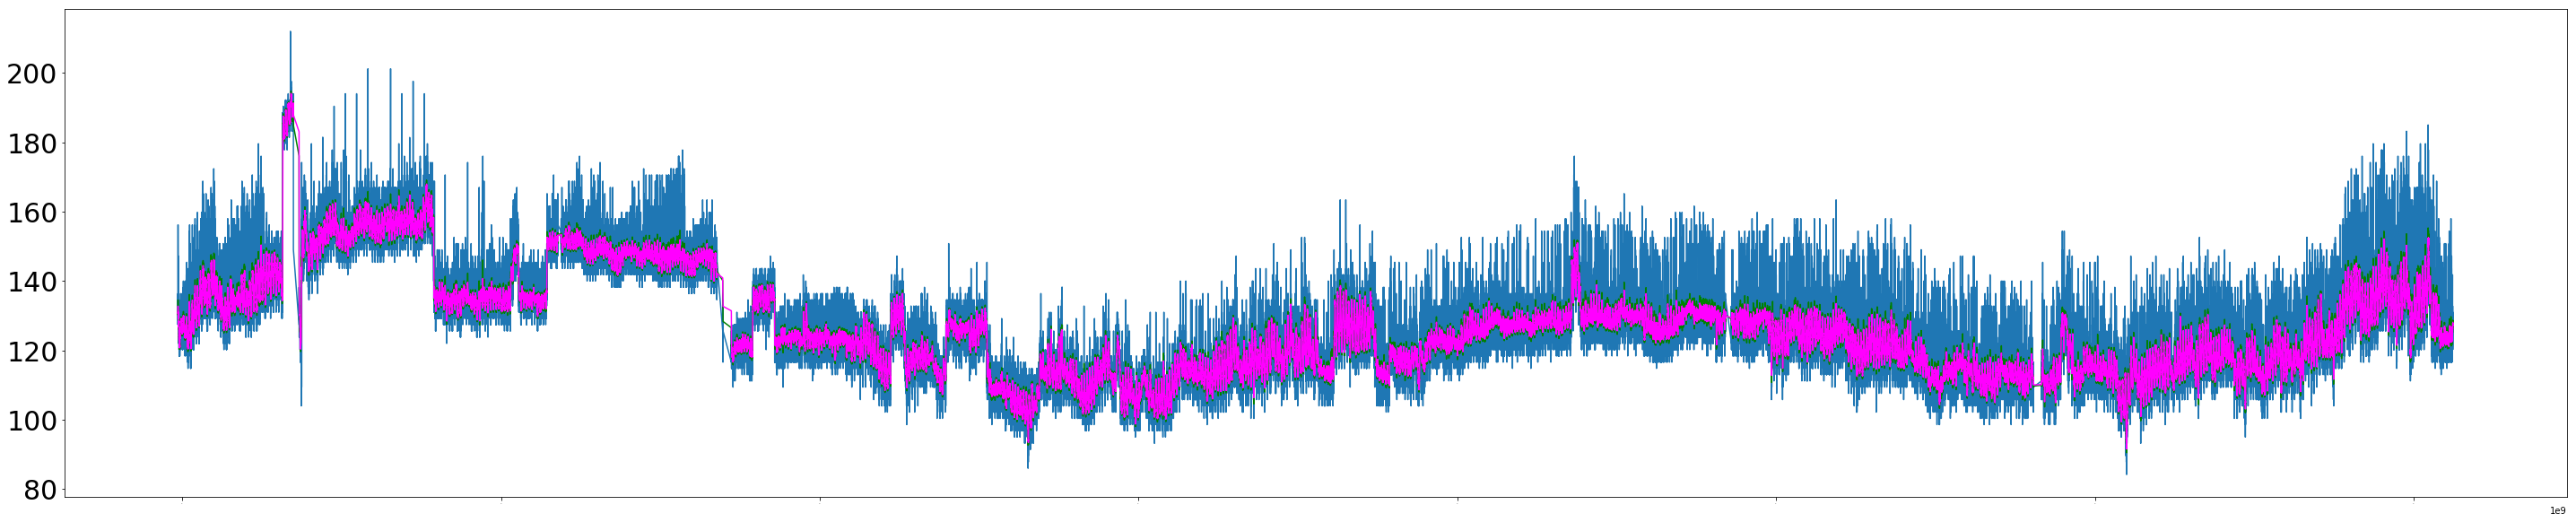
\includegraphics[width=\textwidth]{figures/time_series.png}
\caption{The time series of CPU temperature in the edge cloud deployed at Sedgwick Natural Reserve from Feb. 28th, 2018 to Jun. 3rd, 2020. The x-axis is the epoch time and the y-axis is the CPU temperature in Fahrenheit. } \label{fig:time_series}
\end{figure}

In this work, we propose a heat budget-based scheduling system, \textbf{Sparta}, and investigate its efficacy to control the CPU power dissipation process and prevent CPU temperature from surpassing the preset threshold. In particular, we study the relationship among CPU frequency, temperature, power dissipation and execution pattern, based on which we adopt three modes for Sparta's scheduler. Under the condition that the CPU temperatures are within the threshold, Sparta strives to harness the seasonality of ambient temperature and minimize the execution time of application.

Sparta takes an application, corresponding dataset and a preset temperature threshold as inputs and automatically schedules the workload based on the online sampling temperature data. We use the system to perform a range of machine learning algorithms, including image recognition, natural language processing, decision forest and time series prediction. They comprehensively represent different execution pattern of machine learning application that we utilize in the real-world scenarios.

We build three modes within Sparta's scheduler: \textbf{Annealing} leverages epsilon-greedy strategy to extrapolate the proper CPU frequency in real time; \textbf{AIMD} combines linear growth of CPU frequency when temperature is under threshold with an exponential reduction when it detects any temperature anomaly; \textbf{Hybrid} consolidates Annealing and AIMD modes to overcome their drawbacks and maximizes the efficiency of scheduler. Our results show that Sparta in Hybrid mode speeds up the execution of applications by \textbf{1.16x} and \textbf{1.14x} on average in three thermal environments compared to Annealing and AIMD. In the meantime, Sparta in Hybrid mode has \textbf{94.4\%} of CPU temperature samples remain under the preset threshold on average across all six benchmarks. 

In summary, with this paper, we make the following contributions:

\begin{itemize}
    \item We investigate the relationship between CPU frequency and sampling temperature to precisely model and manage processor power dissipation during execution;
    \vspace{1mm}
    \item We design and implement a heat budget-based scheduling framework that protects edge cloud from overheating and potential damage;
    \vspace{1mm}
    \item We empirically evaluate the efficacy of using Sparta to control CPU temperature and accelerate machine learning applications on six real-world benchmarks in three thermal spectra. 
\end{itemize}

In the following sections, we first discuss the related work (Section~\ref{sec:relate_work}). We then present the design and implementation of Sparta (Section~\ref{sec:Sparta}), following by our experimental methodology and empirical evaluation of the system and application workloads in three different thermal environments (Section~\ref{sec:eval}). Finally, we present our conclusions and future work plans.

\section{Background}
\label{spt:background}
\input{background}

\section{Sparta}
\label{spt:Sparta}
\begin{figure}[ht]
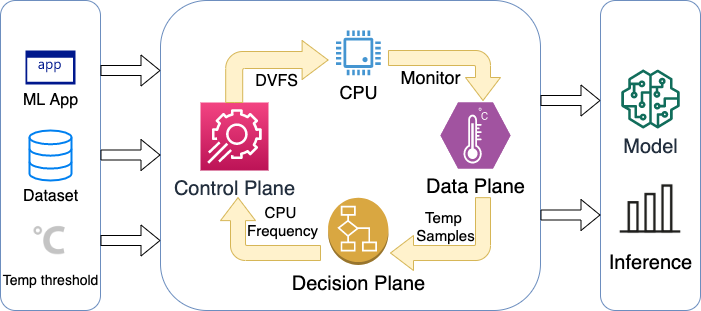
\includegraphics[width=\textwidth]{figures/Sparta.png}
\caption{The Architecture of Sparta} \label{fig:sparta}
\end{figure}

\subsection{Architecture}

To address the processor overheating challenge and accelerate the execution of applications under a CPU temperature threshold, we develop Sparta, a heat-budget-based scheduling framework for edge devices and machine learning applications. The architecture of Sparta is shown in Figure~\ref{fig:sparta}. The scheduler consists of three components: a control plane, a data plane, and a decision plane. Sparta takes a machine learning application, datasets, and a CPU temperature threshold as input. During the execution, the scheduler utilizes a feedback control mechanism that controls the CPU temperature by dynamically adjusting CPU frequency via system-level dynamic voltage and frequency scaling (DVFS). Sparta returns the trained model and inference results at the end of the execution. 


The data plane monitors, samples, and records the CPU real-time temperature via the lm-sensors interface~\cite{ref:sensors} and selects the maximum temperature within a sliding time window. Both the sampling rate and window size are configurable. (1/second and 5 seconds by default) To signify the authentic temperature of multi-core processors, data plane records the temperature samples of the entire CPU package instead of any specific ones. Being accessible by decision plane, all structured temperature data helps determine the proper CPU frequency in real time to keep the CPU temperature under threshold.

The control plane manages the CPU power and temperature. In the design phase, we consider two methods: Sleep injection and DVFS. The first method injects sleep time in the iteration loop that lowers the CPU usage, whereas the second method adjusts the CPU frequency by tuning the CPU voltage. We experiment with these two methods on a multi-threaded matrix multiplication benchmark and monitor the CPU temperature. Figure~\ref{fig:sleep} shows the CPU temperature time series using these two methods. We observe the latter method generates a controllable and stable temperature curve, and thus choose DVFS as the control plane interface. Upon the execution of scheduler, control plane receives the determined CPU frequency and sets the max clock speed of all cores in the CPU package on-the-fly. This way the control plane effectively manages the power consumption and heat generation of the processor.

\begin{figure}[ht]
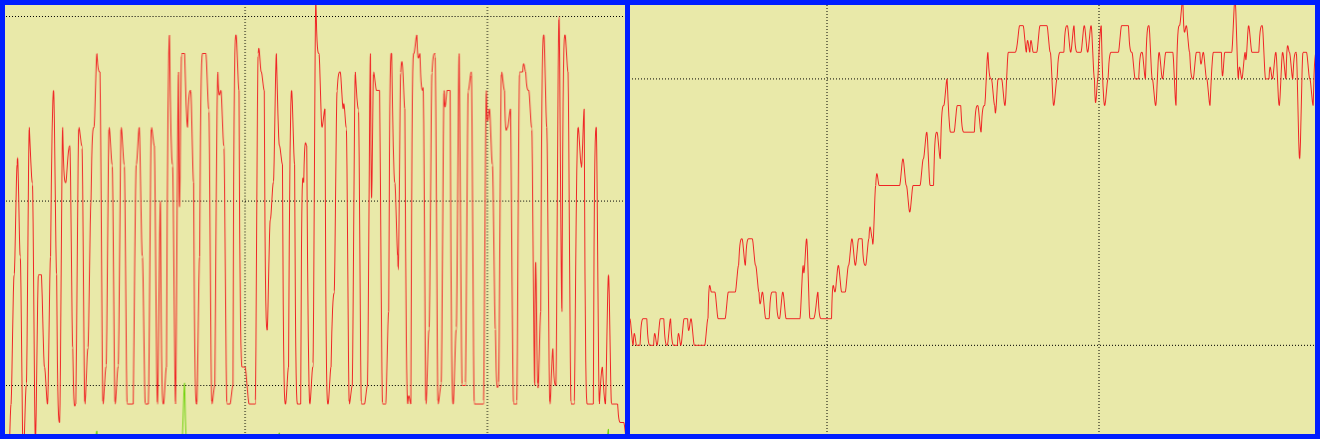
\includegraphics[width=\textwidth]{figures/Sleep-vs-dvfs.png}
\caption{The CPU temperature time series by sleep injection (left) vs DVFS (right). The x-axis is the time frame and the y-axis is the CPU temperature ranging from 48 \degree C to 100 \degree C. } \label{fig:sleep}
\end{figure}


The decision plane
 determines the CPU frequency based on historical and real-time temperature data throughout the execution. To provide the historical dataset, on which decision plane decides the initial CPU frequency, we collect CPU temperature and frequency data from a multi-threaded matrix multiplication (MATMUL) benchmark that simulates the underlying operations in machine learning applications. 

We gather the data in the ambient temperature ranging from 2.6 \degree C to 43.8 \degree C to cover different thermal environments. In the experiment, we found the sequence of CPU frequency and maximum temperature in a time window demonstrate a better linear relationship than the sequence of all temperature, because of its inherent oscillating feature. To verify the correlation between MATMUL and machine learning applications, we collect the same data from an image recognition application written in Tensorflow~\cite{ref:tensorflow}. As depicted in Figure~\ref{fig:mat-vs-tf}, we found the correlated linear relationship between the CPU frequency and logarithmic delta temperature defined as $log(T_{max} - T_i)$, where $T_{max}$ is the maximum temperature sample in the time window and $T_i$ is the starting CPU temperature in idle state. 
 
 Depending on this correlation, decision plane extrapolates the appropriate CPU frequency by linear regression from the MATMUL dataset and assigns initial CPU frequency before the execution starts. During the process, decision plane starts to extrapolate CPU frequency from real-time data that accurately reflects the ambient temperature and the execution pattern of ML applications. The extrapolation frequency is 12/minute by default and configurable by users.

\begin{figure}[ht]
\centering
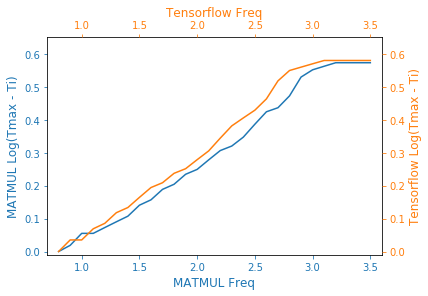
\includegraphics[scale=0.5]{figures/matmul-tensorflow.png}
\caption{The linear relationship between CPU frequency and logarithmic delta temperature of two benchmarks. The blue curve represents MATMUL and the orange curve represents the image recognition application. The plateaus at the right side of curves are caused by CPU hardware temperature throttling. } \label{fig:mat-vs-tf}
\end{figure}


\subsection{Operating Modes}

In the testing phase of Sparta, we identified two major problems in the decision plane. First, the extrapolation from linear regression oftentimes gets stuck at a local minimum. Thus, the determined CPU frequency is frequently lower than the ideal one, which leaves computational resources idle during execution. Second, the response time to correct the CPU from overheating is longer than expected when CPU temperature surpasses the threshold. To solve these two problems, we construct three operating modes for Sparta: Annealing, AIMD, and Hybrid. 

\subsubsection{Annealing} is a probabilistic algorithm that leverages the epsilon-greedy strategy that balances exploration and exploitation by choosing randomly. In this mode, Sparta scheduler picks a value(P) in the range [0, 1] uniformly at random and compares it with $\epsilon/K$, where $\epsilon$ is a probability of taking random actions (0.5 by default) and $K$ is the number of extrapolation decision plane has made. The scheduler assigns a random CPU frequency when P is greater, whereas it keeps the extrapolated frequency when P is less than $\epsilon/K$. With a decreasing probability of $\epsilon/K$ as the application proceeds, scheduler stabilizes and chooses to exploit what it has learned so far. When the ambient temperature or the execution pattern shifts dramatically, the scheduler resets the $\epsilon/K$ that allows more random exploration. This mode effectively addresses the problem of CPU frequency stuck at a local minimum and expedites the execution of machine learning applications under temperature threshold.

\subsubsection{AIMD} is a feedback control mechanism that responds to CPU temperature anomaly faster. The scheduler configures the CPU frequency according to the historical data extrapolation at the start of execution. During the execution, it decreases the CPU frequency by a multiplicative factor (0.5 by default) when CPU temperature surpasses the threshold. Subsequently, it increases the frequency by a fixed amount (0.07 GHz by default) every iteration until the CPU temperature stabilizes right below the threshold. The decision plane turns into hibernation at this point to prevent redundant tuning on CPU frequency that leads to inefficient execution. Meanwhile, the data plane keeps monitoring the CPU temperature and wakes up decision plane if any anomalies caused by ambient temperature or execution pattern are detected. AIMD reduces the response time to temperature deviation and keeps most samples under the threshold. 

\subsubsection{Hybrid} combines Annealing and AIMD modes to address each other's disadvantage: if the probabilistic actions in Annealing drive CPU temperature above threshold, AIMD brings the anomaly back to normal fast; when AIMD settles at a local minimum of CPU frequency and leaves resources idle, Annealing boosts the execution by assigning a random CPU frequency. This way, Hybrid mode provides a complement to accelerate the machine learning execution while keeping the CPU temperature under threshold. 


\section{Evaluation}
\label{spt:eval}
In this section, we empirically evaluate Sparta's performance in a series of experiments on six benchmarks, ranging from image recognition, natural language processing to random forest and time series prediction. We implemented applications based on Tensorflow and executed through Sparta's actuator interface.  In each experiment, Sparta takes inputs of task program, workload dataset and threshold temperature. There are two goals of scheduling by Sparta: the first is to limit the CPU temperature under the threshold; secondly, Sparta accelerates the task to the fullest extent without overheating the edge cloud devices.

\subsection{Machine Learning Benchmarks}

To comprehensively evaluate the efficacy and efficiency of Sparta, we implemented 6 machine learning benchmarks, which consist of four categories: image recognition, natural language processing, ensemble learning and time series analysis. We aim to test Sparta on a variety of machine learning applications that represent different execution patterns.

\subsubsection{WTB\_Train}

is the first image recognition application that we use as a benchmark trains a convolutional neural network (CNN)~\cite{ref:cnn} on the top of ResNet50~\cite{ref:resnet}. The training dataset contains animal images from a wildlife monitoring system called "Where's The Bear" (WTB)~\cite{ref:wtb}. "Where's The Bear" is an end-to-end distributed data acquisition and analytical system that automatically analyzes camera trap images collected by cameras sited at the Sedgwick Natural Reserve~\cite{ref:sedgwick} in Santa Barbara County, California. In total, there are five classes that we consider: Bear, Coyote, Deer, Bird and Empty, by which we label images for training tasks. We also up-sampled minority classes using the Keras Image Data Generator~\cite{ref:datagen}, since the class size is unbalanced due to the frequency of animal occurrences. Doing so ensures that the classification model is not biased. We resized every image in the dataset to $1920 \times 1080$, and for each class, the dataset contains 251 images used to train the CNN model. Once the training is complete, the application stores this model in hdf5 format in object storage. 

The WTB\_Train application has a cold start at the beginning of the execution, since it loads a neural network model and a large dataset. Once it completes loading, the entire training process has relatively consistent CPU usage and temperature. 

\subsubsection{WTB\_Inf}

Based on WTB\_Train, we inference the type of wildlife in camera trap pictures by the second application. It loads the trained model from WTB\_Train and, for each picture, it assigns probabilities to five classes we consider in the training dataset by Softmax function. In terms of the execution pattern, WTB\_Inf runs in short bursts compared to WTB\_Train. Therefore, the CPU usage and temperature fluctuate dramatically throughout the execution of this benchmark.

\subsubsection{MNIST}

 is a dataset containing grayscale pictures of handwritten digits, in which it has 60,000 examples as training set and 10,000 examples as testing set. Based on the dataset, we train a 2-layer convolutional neural network~\cite{ref:MNIST} and test its accuracy in the third application. In contrast to WTB benchmarks, the size of pictures is smaller ($28 \times 28$) and the model is simplified in MNIST. We aim to evaluate Sparta on an application that includes both training and inference process. 

\subsubsection{BiLSTM} is a sentiment analysis application based on a dataset of the Internet Movie Database (IMDB) movie reviews. It consists of 25,000 sequences each for training and testing. The model is constructed as a bidirectional LSTM with a classification layer using sigmoid activation function. We train the model by the training dataset and validate by testing dataset in BiLSTM application. Since it has a large dataset and a complex model, the execution pattern is long-running and consistent in CPU usage and temperature.


\subsubsection{Decision\_Forest} is an implementation of deep neural decision forests~\cite{ref:decision_forest} that classifies high-earning individuals from the pool. The benchmark leverages the United States Census Income Dataset~\cite{ref:uci} that has 48,843 instances with 14 features, including age, education, occupation, etc. The dataset is split up that the training part has 32,561 instances and the testing part has 16,282 instances. The application has three phases: it firstly processes the dataset by encoding input features. Then, it trains a deep neural decision tree model. Based on that, the application trains a neural decision forest model consists of a set of neural decision trees. Therefore, the usage and temperature of CPU increasingly grows throughout the process.


\subsubsection{Time\_Series} is a time series prediction application built on the climate data recorded by the Max Planck Institute for Biogeochemistry~\cite{ref:jena}. The dataset has 14 features such as temperature, pressure, humidity, etc. and the sampling frequency is 10 minutes. The time frame of the dataset ranges from Jan. 10th, 2009 to Dec. 31st, 2016. The application uses 300,693 rows to train a single-layer LSTM model, by which we can predict temperature in next 72 timestamps (12 hours) given the temperature in the past 720 timestamps (120 hours). We intend to evaluate Sparta on an application with light model and large dataset.


% Execution pattern table

\subsection{Experimental Setup}


 

\section{Related Work}
\label{spt:relate_work}
As related work, we consider recent advances in edge cloud's energy consumption and power management.~\cite{ref:computational_sprint} proposes computational sprinting which is a class of mechanisms that supplies additional power on processors for short duration to improve performance. It also introduces phase change materials onto processors to absorb additional heat primarily concerning the performance. ThriftyEdge~\cite{ref:thrifty_edge} presents a resource-efficient edge computing paradigm that consists of an offloading mechanism based on delay-aware task graph partition and a virtual machine selection method. To augment existing resources, \cite{ref:fog} manifests a dynamic fog computing framework that schedules computing tasks to Citizen Fog (CF) with the highest computational ability. Different from the above systems, Sparta focuses on preventing CPU overheating caused by ambient temperature and program execution patterns on edge cloud deployed in natural conditions. 

By offering distributed, reliable, and low-latency machine learning services, edge-based ML as a fast-growing area has a great appeal both for AI and system research community. Thus, we also consider the cutting-edge development in machine learning based on edge cloud. \cite{ref:wireless} explores the building blocks and principles of wireless intelligence at edge networks concerning latency reduction, reliability guarantees, scalability enhancement, and privacy constraints. \cite{ref:survey} provides a comprehensive survey of techniques in the scope of machine learning system at the network edge, including distributed training and inference, real-time video analytics and speech recognition, autonomous vehicles and smart cities, etc. \cite{ref:stargazer} presents an approach to estimate the performance of ML application on edge cloud and to load appropriate computing resources for an edge-based application. The above work provide guiding principles and examples for Sparta and serve as one of the key motivations for our work.


\section{Conclusion}
\label{spt:conclusion}
In this paper, we propose a heat budget-based scheduling framework, called Sparta, aiming to prevent edge cloud CPU overheating in executing machine learning applications. Sparta's scheduler integrates three components -- data plane, decision plane, and control plane: Decision plane extrapolates the initial CPU frequency from historical benchmark data and dynamically adjusts it based on real-time data monitored by data plane, while control plane modified the CPU frequency via DVFS throughout the execution. Sparta strives to accelerate the execution of applications without sacrificing the CPU overheating protection.  

We present the design principles and implementation details of Sparta's components and operating modes that address the drawback we encounter in the testing phase. Our empirical evaluation demonstrates Sparta effectively protects CPU from overheating, putting \textbf{94.4\%} temperature samples under the threshold in Hybrid mode. In the meantime, it speeds six benchmarks' execution up to \textbf{1.04x} - \textbf{1.32x} in all three thermal environments compared to Annealing and AIMD.

As part of future work, we plan to investigate using non-uniform distributions in generating random values for exploration in Annealing mode that potentially improves the PTBT metrics. We also plan to extend the deployment of Sparta at edge cloud clusters and investigate its performance in the distributed execution of training and inference process. 


%
% ---- Bibliography ----
%
% BibTeX users should specify bibliography style 'splncs04'.
% References will then be sorted and formatted in the correct style.
%

% \bibliographystyle{splncs04}
% \bibliography{ref}

\begin{thebibliography}{8}

\bibitem{ref:wtb}
A. R. Elias, N. Golubovic, C. Krintz and R. Wolski, "Where's the Bear? - Automating Wildlife Image Processing Using IoT and Edge Cloud Systems," 2017 IEEE/ACM Second International Conference on Internet-of-Things Design and Implementation (IoTDI), pp. 247-258, 2017.

\bibitem{ref:sedgwick}
Sedgwick Natural Reserve Homepage \url{https://sedgwick.nrs.ucsb.edu} Last accessed 30 Apr 2021

\bibitem{ref:cnn}
Yann LeCun and Yoshua Bengio. Convolutional networks for images, speech, and time series. The handbook of brain theory and neural networks. MIT Press, Cambridge, MA, USA, pp. 255–258, 1998.

\bibitem{ref:datagen}
Keras Image Data Generator \url{https://keras.io/preprocessing/image/\#imagedatagenerator-class} Last accessed 30 Apr 2021

\bibitem{ref:resnet}
He, Kaiming, Xiangyu Zhang, Shaoqing Ren, and Jian Sun. "Deep residual learning for image recognition." In Proceedings of the IEEE conference on computer vision and pattern recognition, pp. 770-778. 2016.

\bibitem{ref:MNIST}
Y. LeCun, L. Bottou, Y. Bengio and P. Haffner: Gradient-Based Learning Applied to Document Recognition, Proceedings of the IEEE, 86(11):2278-2324, November 1998

\bibitem{ref:decision_forest}
P. Kontschieder, M. Fiterau, A. Criminisi and S. R. Bulò, "Deep Neural Decision Forests," 2015 IEEE International Conference on Computer Vision (ICCV), 2015, pp. 1467-1475, \doi{doi: 10.1109/ICCV.2015.172}.

\bibitem{ref:uci}
\url{https://archive.ics.uci.edu/ml/datasets/census+income} Last accessed 30 Apr 2021

\bibitem{ref:jena}
\url{https://www.bgc-jena.mpg.de/wetter/} Last accessed 30 Apr 2021 

\bibitem{ref:nuc}
\url{https://www.intel.com/content/www/us/en/products/boards-kits/nuc.html} Last accessed 30 Apr 2021 


\bibitem{ref_proc1}
Author, A.-B.: Contribution title. In: 9th International Proceedings
on Proceedings, pp. 1--2. Publisher, Location (2010)

\end{thebibliography}

\end{document}
